\sectionsansnumero{Introduction}
	Ce PRT consiste en la création d'une carte de développement pouvant servir de base à d'autres projets en électronique.
    Ne constituant pas un objet très intéressant du point de vue des diverses analyses, cette carte est vue comme l'élément central d'un poste de radio portatif multiprotocole.
     Ainsi, les différents schémas sont réalisés avec cette carte comme étant l'élément principal, mais le produit vendable est le poste de radio.
     Nous ferons donc une partie de l'analyse fonctionnelle externe ainsi que l'analyse de la concurrence pour la carte électronique au sein de la radio puis nous considérerons uniquement la carte électronique pour la suite de l'analyse.
     
     Ce document est donc structuré en trois parties~:
    \begin{itemize}
	    \item Partie 1~: Le cahier des charges fonctionnel délimite le produit et son usage.
        \item Partie 2~: La démarche de développement présente les aspects plus techniques du projet.
        \item Partie 3~: L'organisation situe la coordination des différentes étapes de la création du produit ainsi que l'analyse des risques associés.
    \end{itemize}
    
\section{Cahier des charges fonctionnel}
	\subsection{Approche marché}
    	Pour pouvoir trouver sa place dans un environnement de plus en plus connecté, un poste de radio doit proposer les fonctionnalités attendues de récupération de contenu tels que les webradios ou la radio numérique (DAB) en plus des fonctionnalités classiques AM/FM.
        Les principaux aspects de ce produit sont donc un design élégant et minimaliste ainsi qu'une grande compatibilité avec les différents protocoles de diffusion de radio (hertzienne ou internet).
        Cet objet doit également être facile à utiliser, en offrant une interface unifiée à l'utilisateur ainsi que de fonctionnalités intelligentes avancées facilement utilisables et transparentes de son point de vue.
        
    \subsection{Cible et positionnement visés}
    	La clientèle ciblée est la jeune génération, en recherche de connectivité, de simplicité dans l'usage des technologies modernes.
        Le produit est ainsi pensé avec un design soigné et réaliser correctement sa fonction, sans complexité inutile.
        Le prix ne doit pas être trop élevé, car ce produit ne vise pas les applications hautes-fidélités, mais doit attirer grâce à sa simplicité.
        
    \subsection{Analyse fonctionnelle externe}
    	Cette partie introduit l'analyse fonctionnelle externe du poste de radio.
        Plusieurs diagrammes tels que la bête à cornes, le cycle de vie ou encore le diagramme pieuvre sont présentés.
        Le projet de PRT est au départ une carte de développement générique et dépourvue de fonctionnalités avancées. Cette analyse fonctionnelle est donc celle de cette carte, mais remise dans un contexte où elle servirait de base pour la conception d'un poste de radio portatif multiprotocole. 
    
    	\subsubsection{Bête à Cornes}
        Le besoin et l'objectif du projet sont exprimés avec la bête à cornes suivante :
        	\inclurepdf{Bête à Cornes}{BeteACorne}{PDF/BeteACorne.pdf}

        \subsubsection{Diagramme Pieuvre}
        	Le diagramme pieuvre renseigne sur les blocs principaux du produit, ainsi que leurs relations de contraintes et la fonctions qu'ils doivent remplir.
            \inclurepdf{Diagramme Pieuvre}{DiagrammePieuvre}{PDF/Pieuvre.pdf}
			% Usage de sidewaystable au lieu de table pour mettre le tableau en paysage
\begin{sidewaystable}[H]
% Group for vertically centered cells
\begingroup{}
% Use vertically centered cells
\def\tabularxcolumn#1{m{#1}}

\begin{tabularx}{\textwidth}{|X|X|X|X|X|}
\hline
\rowcolor[HTML]{5B9BD5} 
    & Fonctions de service
    & Critères d'évaluations
    & Niveau d'exigence
    & Flexibilité
    \\ \hline
FP1
  & Envoyer le signal sonore amplifié vers les haut-parleurs
  & Puissance et qualité du son 
  & 2x3W, son 'chaud' et non saturé
  & F0 \newline Puissance~:±1W 
  \\ \hline

\rowcolor[HTML]{ACCCEA} 
FP2
  & Être alimentée par le secteur ou une batterie  et disposer d'une autonomie intéressante le cas échéant
  & Bonne autonomie 
  & 20h d'autonomie
  & F0
  \\ \hline
  

FC1
  & Traiter les informations
    provenant de l'écran tactile et des boutons
  & Faible latence et fluidité des contrôles
  	\newline Minimalisme des commandes possibles 
    
  & Moins de 100 ms entre l'appui et la réponse 
  & F1 \newline Latence~: ±20ms
  \\ \hline

\rowcolor[HTML]{ACCCEA} 
FC2
  & S'intégrer au boitier en n'altérant pas le design de l'objet 
  &            
  & 
  & 
  \\ \hline
  
FC3
  & Etablir une connectivité et traiter les informations provenant de l'application compagnon
  & Faible latence et fluidité des contrôles
    \newline Portée importanteMinimalisme des commandes possibles
  & Moins de 100 ms entre l'appui et la réponse.
    \newline Portée de 40m en indoor
  & F1 \newline Latence~: ±20ms \newline Portée~: ±15m
  \\ \hline

\rowcolor[HTML]{ACCCEA} 
FC4
  & Respect des différentes normes en vigueur
   \newline Normes CE principalement~:
   \newline Compatibilité électromagnétique (CEM) - 2014/30/UE 
   \newline et Équipements terminaux de télécommunication - 1999/5/CE

  & Respect des normes 
  & Toutes les normes doivent être respectées 
  & F0 
  \\ \hline
  
FC5 
  & Traiter les données provenant du tuner  
  & Traitement rapide et sans perte 
  & Pas de pertes de données 
  & F0
  \\ \hline
  
\end{tabularx}
\endgroup{}
\caption{Fonctions principales et de contraintes}
\end{sidewaystable}
            
            \subsubsection{Cycle de vie}
        	Le cycle de vie du produit permet de ne pas oublier d'élément de l'environnement dans lequel notre produit va évoluer durant sa durée de vie.
            \inclurepdf{Cycle de vie}{CycleDeVie}{PDF/CycleDeVie.pdf}
            
    \subsection{Analyse de la concurrence}
    	Pure et Sagem sont les acteurs principaux de ce marché. Avec deux modèles principaux vendus respectivement à 100\euro{} et 111\euro{}.
        Logitech s'est rétractée de ce marché après avoir sorti un modèle à plus de 300\euro{} en 2012. 
\\Le Sagem RM50 offre un design extrêmement sobre, très classique avec une douzaine de boutons de contrôle.
Il présente quelques fonctionnalités "smart" mais celles-ci restent limitées. Aucune application smartphone compagnon n'est proposée.
Il n'a pas de batterie, donc aucune possibilité de nomadisme. Il manque également un port USB pour la lecture du contenu personnel.
Autrement les retours sont globalement bons sur ce produit.

Le Pure One Flow est plus compact, il présente un design également très sobre et très classique.
Cependant la batterie est proposée en option à un prix relativement élevé.
Les retours ne sont pas particulièrement bons sur ce produit~: les commandes sont complexes, l'assemblage de mauvaise qualité, mais le produit remplit correctement sa fonction.

Le design que nous souhaitons proposer, les solutions simples et intégrées, les fonctionnalités dites "smart" que nous souhaitons proposer ainsi que le prix sont donc nos principaux éléments de différenciation.
        
    \subsection{Principes technologiques imposés}
		La carte de développement doit fournir les outils de base permettant à un concepteur de tester des idées, afin d'accélérer le développement du produit. 
    	Elle est constituée d'un microcontrôleur permettant d'utiliser un système d'exploitation GNU/Linux.
        Pour arriver à cet objectif, la carte possède également de la mémoire de stockage de masse (mémoire NOR) ainsi que de la RAM externe au micro contrôleur. 
        Quelques périphériques seront exploités, comme un port USB OTG High Speed, un écran tactile et un bus à choisir pour lequel un pilote sera développé.
        Étant un sujet proposé par le binôme, le cahier des charges est souple, l'objectif principal du projet étant la confrontation aux différents problèmes que l'on rencontre dans la mise en œuvre de ces technologies.
        
\section{Démarche de développement}

	\subsection{Phasage}   	 
     Le diagramme de phasage donne un aperçu des différentes phases de développement en listant les tâches principales associées.     
     \inclurepdf{Phasage du projet}{Phasage}{PDF/Phasage.pdf}
     
    \subsection{Choix de conception}
    	Le choix de réaliser une carte à base d'un microcontrôleur ARM Cortex M4 (STM32F429) vient de la volonté de concevoir une carte de développement supportée par le noyau Linux. Une carte basée sur un ARM Cortex A a été envisagé, mais l'idée a été rejetée à cause de la difficulté technique (boîtier du composant en BGA très délicat à souder manuellement, bus haute fréquence, etc.).
        En revanche, le microcontrôleur choisi est bon marché et est suffisamment simple pour être manipulé et débuggé avec les moyens à disposition.
        L'usage du noyau uClinux au lieu du noyau Linux standard est dû aux caractéristiques techniques du microcontrôleur (absence de Memory Management Unit).
       
       Afin de pouvoir satisfaire les besoins d'un tel système, il est indispensable d'inclure une mémoire de masse (mémoire NOR) ainsi que une extension externe de mémoire vive (SDRAM).
        Un écran LCD tactile et un port USB seront ajoutés au projet, afin de pouvoir réaliser des démonstrations plus attractives.
       
       	D'un côté pédagogique, un bus relativement simple (I2C ou SPI) sera exploité par le biais de l'écriture d'un pilote pour uClinux.
    	Enfin, un port SWD sera utilisé pour le débogage.
        
    \subsection{Organigramme technique}
    	Le diagramme technique illustre les principaux blocs que l'on retrouve sur la carte de développement et leurs interactions~:
    	\inclurepdf{Schéma-bloc de la carte de développement}{SchemaBloc}{PDF/Bloc_Diagram_PRT.pdf}
      	
      
\section{Organisation}
	\subsection{Planning Gantt}
    	Le planning de Gantt permet de repérer le découpage en tâche du travail à faire et de le répartir sur le temps imparti.
        Sa limite est la connaissance de la durée des étapes, ainsi que des problèmes susceptibles d'apparaître.
    
	    \begin{figure}[H]
			\centering
            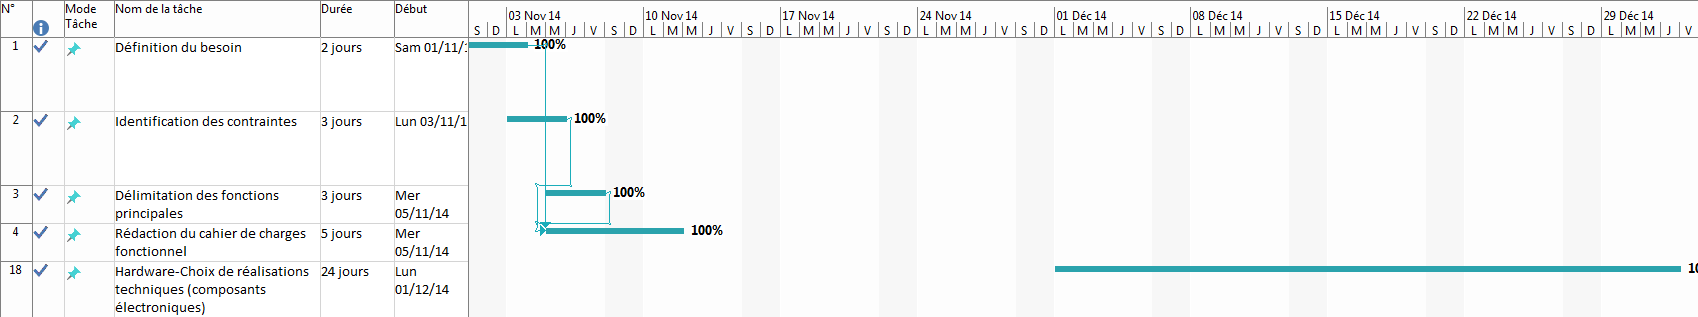
\includegraphics[angle=90,scale=0.33]{Gantt/gantt1.png}
            \caption{Diagramme de Gantt, partie 1}
		\end{figure}
        
	    \begin{figure}[H]
			\centering                    
    	    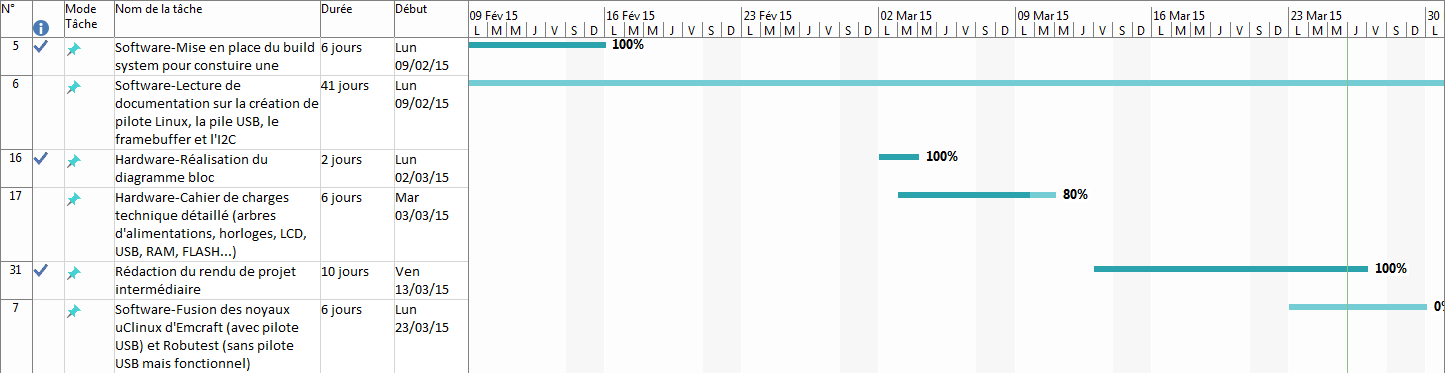
\includegraphics[angle=90,scale=0.5]{Gantt/gantt2.png}
            \caption{Diagramme de Gantt, partie 2}
		\end{figure}

	    \begin{figure}[H]
			\centering
      		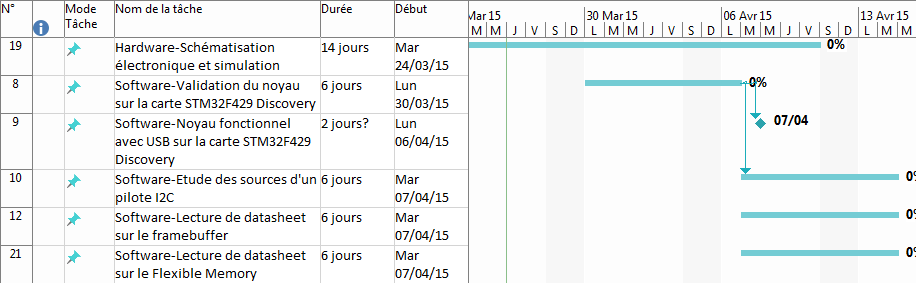
\includegraphics[angle=90,scale=0.7]{Gantt/gantt3.png}
            \caption{Diagramme de Gantt, partie 3}
		\end{figure}

	    \begin{figure}[H]
			\centering
     		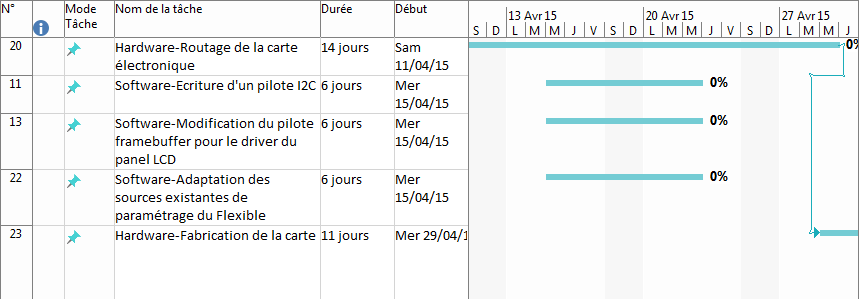
\includegraphics[angle=90,scale=0.8]{Gantt/gantt4.png}
            \caption{Diagramme de Gantt, partie 4}
		\end{figure}

	    \begin{figure}[H]
			\centering
            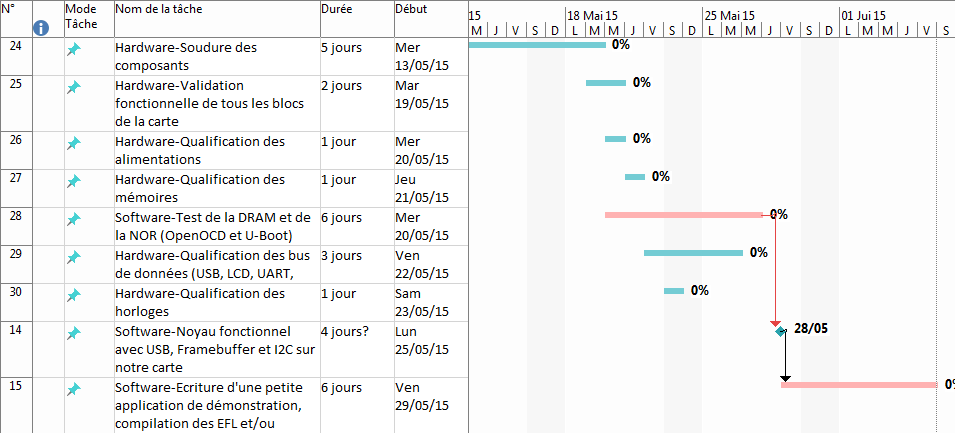
\includegraphics[angle=90,scale=0.6]{Gantt/gantt5.png}
            \caption{Diagramme de Gantt, partie 5}
		\end{figure}
        
        
    \subsection{Jalon de fin de phase}
    	Les différentes phases sont marquées par un accomplissement validant les étapes intermédiaires.
        Ces jalons sont importants pour s'assurer que les fonctions mises en \oe uvre dans une étape sont opérationnelles avant d'implémenter des fonctions qui en dépendent~:
    	\begin{itemize}
      		\item La rédaction du cahier des charge
            \item La définition des interfaces de la carte (I/O)
            \item La schématisation et le routage de la carte
            \item La validation des fonctions de base (CPU, mémoires) grâce au bootloader et à la sonde de debug
            \item La validation des fonctions plus complexes (écran LCD, USB)
            \item Validation du système entier (application, espace utilisateur complet final avec BusyBox)
            \item La soutenance finale
      	\end{itemize}
      
    \subsection{Analyse préalable des risques}
    	L'analyse des risques permet d'identifier les principaux problèmes susceptibles de se présenter et la manière de les gérer.
    	% Table generated by Excel2LaTeX from sheet 'Feuil1'
\begin{sidewaystable}[H]
  \centering
  % Group for vertically centered cells
  \begingroup{}
  % Use vertically centered cells
  \def\tabularxcolumn#1{m{#1}}
  
    \begin{tabularx}{\textwidth}{|p{1cm}|X|p{0.5cm}|p{0.5cm}|p{0.5cm}|X|p{2cm}|p{1cm}|}
    \hline
    \rowcolor[HTML]{ACCCEA} 
    N°    & Défaillance potentielle & \begin{sideways}Occurrence\end{sideways} & \begin{sideways}Gravité\end{sideways} & \begin{sideways}Criticité\end{sideways} & Action en prévention ou résolution du risque & Responsable & Délai \\ 
    \hline
    \multicolumn{8}{|l|}{\textbf{I. Phase d'émergence}} \\ \hline
          & Contraintes techniques identifiées trop fortes & \textcolor{yellow}{5}     & \textcolor{green}{3}     & 15      & Revoir les exigences du Cahier de charges à la baisse & Badr B.
Douglas R. & 2j \\ \hline
	
    \multicolumn{8}{|l|}{\textbf{II. Conception}} \\ \hline
          & Composants choisis obsolètes
(plus commercialisés) & \textcolor{green}{3} & \textcolor{red}{15}    & 45      & Prendre en compte les dates de
support données par le fabricant lors du choix & Badr B. & 1j \\ \hline
          & Composants choisis trop chers & \textcolor{green}{3}     & \textcolor{yellow}{5}     & 15      & Prendre en compte le coût des composants lors du choix & Badr B. & 1j \\ \hline
          & Support fabricants faible & \textcolor{green}{3}     & \textcolor{yellow}{5}     &  15     & Choisir des composants à usage relativement
répandus et 'supportés' par une communauté & Badr B. & 1j \\ \hline
          & Mauvais résultats de simulation & \textcolor{yellow}{5}     & \textcolor{red}{15}    & 75      & Revoir le cahier de charges techniques
ou changer de composants & Badr B. & 2j \\ \hline

          & Temps de mise en œuvre prévue d'une fonctionnalité logicielle trop élevée & \textcolor{yellow}{5}     & \textcolor{red}{15}    & 75      & Revoir le cahier de charges & Douglas R. & 2j \\ \hline
    
    \multicolumn{8}{|l|}{\textbf{III. Définition détaillée}} \\ \hline
          & Incompatibilité entre composants
lors de l'intégration & \textcolor{yellow}{5}     & \textcolor{red}{15}    & 75      & Changer de composants & Badr B. & 1j \\ \hline

    \multicolumn{8}{|l|}{\textbf{IV. Réalisation de prototype}} \\ \hline
          & Routage trop complexe & \textcolor{green}{3}     & \textcolor{yellow}{5}     & 15      & Revoir le Gantt et allouer plus de temps au routage & Badr B.
Douglas R. & 1j \\ \hline
          & Problèmes inattendus à débogger & \textcolor{green}{3}     & \textcolor{yellow}{5}     & 15      & Revoir le Gantt et allouer plus de temps au déboggage & Badr B.
Douglas R. & 1j \\ \hline
          & Routage sur 2 couches impossible & \textcolor{yellow}{5}     & \textcolor{yellow}{5}     & 25      & Trouver le meilleur fournisseur pour un routage sur 4 couches & Badr B. & 1j \\ \hline
          & Bill of materials + PCB > 100€ & \textcolor{red}{15}    & \textcolor{yellow}{5}     & 75      & Commandes de samples si possible ou sinon changement de composant
Optimisation du routage (réduction de la surface du PCB)
Négociation d'une rallonge sur le budget du projet & Badr B.
Douglas R. & 3j \\ \hline
    \end{tabularx}%
  \endgroup{}
  \caption{Analyse des risques, partie 1}    
\end{sidewaystable}%


% Table generated by Excel2LaTeX from sheet 'Feuil1'
\begin{sidewaystable}[H]
  \centering
  % Group for vertically centered cells
  \begingroup{}
  % Use vertically centered cells
  \def\tabularxcolumn#1{m{#1}}
  
    \begin{tabularx}{\textwidth}{|p{1cm}|X|p{0.5cm}|p{0.5cm}|p{0.5cm}|X|p{2cm}|p{1cm}|}
    \hline
	\rowcolor[HTML]{ACCCEA}     
    N°    & Défaillance potentielle & \begin{sideways}Occurrence\end{sideways} & \begin{sideways}Gravité\end{sideways} & \begin{sideways}Criticité\end{sideways} & Action en prévention ou résolution du risque & Responsable & Délai \\
    \hline
 \multicolumn{8}{|l|}{\textbf{V. Test et validation}} \\ \hline
          & Echec de la validation fonctionnelle & \textcolor{green}{3}     & \textcolor{red}{15}    & 45     & Identification rapide du problème
(qui peut être dû à de très nombreuses causes)
et prendre les décisions nécessaires & Badr B.
Douglas R. & x \\ \hline
          & Alimentations hors specification & \textcolor{green}{3}     & \textcolor{yellow}{5}     & 15      & Revue du routage ou du dimensionnement des composants & Badr B. & 2j \\ \hline
          & Signaux RAM, NOR, USB, UART, I2C hors specification & \textcolor{yellow}{5}     & \textcolor{yellow}{5}     & 25      & Reprendre le routage ou changer les composants & Badr B.
Douglas R. & x \\ \hline
          & Matériel de mesure non adapté & \textcolor{yellow}{5}     & \textcolor{red}{15}    & 45       & Faire une demande spéciale pour
accéder à de meilleurs équipements & Badr B.
Douglas R. & 1j \\ \hline
    \end{tabularx}%
  \endgroup{}
    
  \caption{Analyse des risques, partie 2}    
\end{sidewaystable}%

        
        
\sectionsansnumero{Conclusion}
	Ce projet est à but avant tout pédagogique, avec pour objectif principal la montée en compétence sur les différentes technologies manipulées (implémentation de microcontrôleurs, mise en \oe uvre de uClinux, développement de pilotes).
    Il est aussi l'occasion de se pencher sur la démarche de développement d'un produit fini sur un projet réaliste.
    L'analyse fonctionnelle permet ainsi de mieux cerner le projet, et de diminuer les risques d'omission d'un aspect important mais pas directement visible au premier abord.

